\chapter{Prelimenaries}

\begin{defn}[H-certificate]
    Graph $H$ is a minor of $G$ if there exists $c := (V_{t})_{t \in V(H)}$ of pairwise disjoint $V(G)$,
     called bags, such that $\forall t \in V(H)$ $V_{t} \neq \emptyset$ and $G[V_{t}]$ is connected, and $\forall (u,v) \in E(H)$,
     $\exists$ edge connecting $V_{u}$ and $V_{v}$, any such $c$ is called $H$-certificate
\end{defn}

\begin{defn}[rooted H-certificate]
    $H$-certificate is a rooted if $V(H) \subset V(G)$ and $t \in V_{t}$ $\forall t \in V(H)$. If there is a rooted H-certificate in graph $G$,
    then $H$ is a rooted minor of $G$
\end{defn}

\begin{defn}[Routing Graph]
Let $\mathcal{C}$ be a coloring of graph $G$, let $T$ be the transversal of coloring $\mathcal{C}$, 
then routing graph $H(G, \mathcal{C}, T)$ is defined as the graph on vertices of $T$, 
such that $\forall (i,j) \in V(H) (i \neq j)$, $(i,j) \in E(H)$ if and only if 
$\exists$ Kempe chain between vertices $i$ and $j$ in graph $G$
\end{defn}

\begin{defn}[Property (*)]
    All graphs $H$ which are routing graph of some $G$ with some coloring $\mathcal{C}$ and transversal $T$
    such that $G$ has a rooted $H$-certificate, are said to have property (*)
\end{defn}

\begin{thm}
\label{thm:1}
    Property (*) inherits to subgraphs of K and K has property (*) if and only if every component of K has it.
\end{thm}

\begin{proof}
    Proved in \cite{matthias_2022} Theorem 1
\end{proof}

\begin{thm}
\label{thm:2}
    Let $K$ be a graph and $q \in V(K)$ and $deg(1) = 1$. If $K - q$ has property (*), then $K$ has property (*).
\end{thm}

\begin{proof}
    Proved in \cite{matthias_2022} Lemma 1
\end{proof}

\begin{thm}
\label{thm:3}
    $K_7$ does not have property (*)
\end{thm}

\begin{proof}
    Proved in \cite{matthias_2022} Theorem 2

    Since by Theorem \ref{thm:1} property (*) inherits to subgraphs of $K_7$, they found a subgraph of $K_7$, $H$, and a graph $G$ with a coloring $\mathcal{C}$ and a transversal $T$ such that 
    $H$ is isomorphic to $H(G, \mathcal{C}, T)$, but $H$ is not a rooted minor of $K_7$.

    \begin{figure}[H]
        \centering
        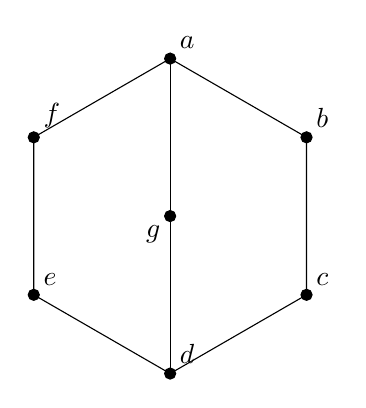
\begin{tikzpicture}[scale=1]
    
            \coordinate (a) at (0,2);
            \coordinate (b) at ({2*cos(30)},{2*sin(30)});
            \coordinate (c) at ({2*cos(-30)},{2*sin(-30)});
            \coordinate (d) at (0,-2);
            \coordinate (e) at ({2*cos(-150)},{2*sin(-150)});
            \coordinate (f) at ({2*cos(150)},{2*sin(150)});
            \coordinate (g) at (0,0);
            
            \draw (a) -- (b) -- (c) -- (d) -- (e) -- (f) -- cycle;
            
            \draw (g) -- (a);
            \draw (g) -- (d);
            
            \foreach \i in {a,b,c,d,e,f}{
                \filldraw (\i) circle (2pt);
                \node[above right] at (\i) {${\i}$};
            }
            
            % Draw x
            \filldraw (g) circle (2pt);
            \node[below left] at (g) {$g$};
            
            \end{tikzpicture}
            \caption{The subgraph of $K_7$ without (*) property}
    \end{figure}

    \begin{figure}[H]
        \centering
        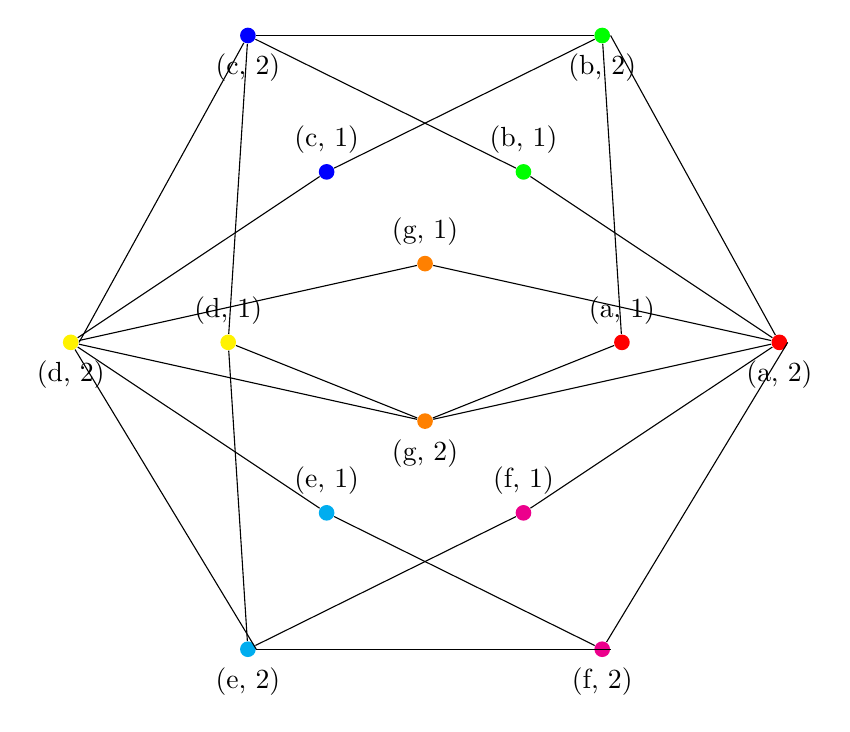
\begin{tikzpicture}
            \def\radius{2.5cm}
            \def\outerradius{4.5cm}
            
            % Add the central vertices (g, 1) and (g, 2) with the same color (orange)
            \node[circle, fill=orange, inner sep=2pt, label=above:{(g, 1)}] (vcenter1) at (0, 1) {}; % Shifted slightly up
            \node[circle, fill=orange, inner sep=2pt, label=below:{(g, 2)}] (vcenter2) at (0, -1) {}; % Shifted slightly down
            
            % Draw the inner circle vertices
            \foreach \i/\color [count=\j from 0] in {(a, 1)/red, (b, 1)/green, (c, 1)/blue, (d, 1)/yellow, (e, 1)/cyan, (f, 1)/magenta} {
                \node[circle, fill=\color, inner sep=2pt, label=above:\i] (v1\j) at ({360/6 * \j}:\radius) {};
            }
            
            % Draw the outer circle vertices
            \foreach \i/\color [count=\j from 0] in {(a, 2)/red, (b, 2)/green, (c, 2)/blue, (d, 2)/yellow, (e, 2)/cyan, (f, 2)/magenta} {
                \node[circle, fill=\color, inner sep=2pt, label=below:\i] (v2\j) at ({360/6 * \j}:\outerradius) {};
            }
            
            % Connect outer circle vertices
            \foreach \j in {0,...,5} {
                \pgfmathsetmacro{\nextj}{mod(\j+1, 6)}
                \draw (v2\j) -- (v2\nextj);
            }
            
            % Connect inner and outer circle vertices
            \draw (v20) -- (v11);
            \draw (v21) -- (v10);
            \draw (v22) -- (v11);
            \draw (v23) -- (v12);
            \draw (v21) -- (v12);
            \draw (v22) -- (v13);
            \draw (v24) -- (v13);
            \draw (v23) -- (v14);
            \draw (v25) -- (v14);
            \draw (v24) -- (v15);
            \draw (v20) -- (v15);
            
            % Connect (g, 2) to (a, 2) and (d, 2)
            \draw (vcenter2) -- (v20); % (g, 2) to (a, 2)
            \draw (vcenter2) -- (v23); % (g, 2) to (d, 2)
            
            % Connect (g, 1) to (a, 2) and (d, 2)
            \draw (vcenter1) -- (v20); % (g, 1) to (a, 2)
            \draw (vcenter1) -- (v23); % (g, 1) to (d, 2)
            
            % Connect (a, 1) to (g, 2) and (d, 1) to (g, 2)
            \draw (v10) -- (vcenter2); % (a, 1) to (g, 2)
            \draw (v13) -- (vcenter2); % (d, 1) to (g, 2)
        \end{tikzpicture}
        \caption{Example of $Z(G)$ given $G$ is $C_7$ with additional connections to $(g, 1)$ and $(g, 2)$.}
        \label{Fig:Main}
    \end{figure}
    In Figure \ref{Fig:Main}, the graph $G$ is shown with coloring
    $\mathcal{C}$ and transversal $T := \{(a, 1), (b, 1), (c, 1), (d, 1), (e, 1), (f, 1), (g, 1)\}$.
\end{proof}

\begin{thm}
    \label{thm:6}
        Every graph on at most four vertices has property (*).
\end{thm}
    
\begin{proof}
        Proved in \cite{matthias_2022} Theorem 4
\end{proof}

\begin{thm}
\label{thm:4}
    Every connected graph with at most one cycle has property (*)
\end{thm}

\begin{proof}
    Proved in \cite{matthias_2022} Theorem 5
\end{proof}

\begin{thm}
\label{thm:5}
    Every graph on five vertices and at most six edges has property (*)
\end{thm}

\begin{proof}
    Proved in \cite{matthias_2022} Theorem 7
\end{proof}
